\documentclass[aspectratio=169,11pt]{beamer}

% ============================================================
% PACKAGES
% ============================================================
\usepackage{graphicx}
\usepackage{tikz}
\usetikzlibrary{positioning,arrows.meta}
\usepackage{xcolor}
\usepackage{booktabs}
\usepackage{tabularx}
\usepackage{array}
\usepackage{ragged2e}
\usepackage{hyperref}
\newcolumntype{R}[1]{>{\RaggedRight\hyphenpenalty=10000\arraybackslash}p{#1}}
\newcolumntype{Y}{>{\RaggedRight\hyphenpenalty=10000\arraybackslash}X}
\newcommand{\ph}[1]{[#1]}

% ============================================================
% COLORS
% ============================================================
\definecolor{GEUBlue}{RGB}{20,55,105}
\definecolor{GEULightBlue}{RGB}{238,244,251}
\definecolor{GEUGrey}{RGB}{90,90,90}
\definecolor{GEULightGrey}{RGB}{245,246,248}

% ============================================================
% BEAMER SETTINGS
% ============================================================
\usetheme{default}
\setbeamertemplate{navigation symbols}{}
\setbeamertemplate{blocks}[rounded][shadow=false]

\setbeamercolor{normal text}{fg=black,bg=white}
\setbeamercolor{frametitle}{fg=GEUBlue}
\setbeamercolor{structure}{fg=GEUBlue}
\setbeamercolor{block title}{fg=GEUBlue,bg=GEULightBlue}
\setbeamercolor{block body}{fg=black,bg=GEULightBlue}

\setbeamerfont{frametitle}{size=\Large,series=\bfseries}
\setbeamerfont{itemize/enumerate body}{size=\small}
\setbeamerfont{itemize/enumerate subbody}{size=\footnotesize}
\setlength{\leftmargini}{1.2em}
\setlength{\parskip}{0pt}

% ============================================================
% LOGO
% ============================================================
\newcommand{\GEULogo}{media/graphicera_logo.png}

% ============================================================
% HEADER
% ============================================================
\setbeamertemplate{headline}{%
  \begin{tikzpicture}[remember picture,overlay]
    \node[
        anchor=north east,
        xshift=-0.30cm,
        yshift=-0.12cm
    ] at (current page.north east)
    {\includegraphics[height=0.62cm]{\GEULogo}};
  \end{tikzpicture}
  \vspace{0.55cm}
}

% ============================================================
% FRAME TITLE
% ============================================================
\setbeamertemplate{frametitle}{%
  \vspace{0.03cm}
  {\usebeamercolor[fg]{frametitle}\usebeamerfont{frametitle}\insertframetitle\par}
  \vspace{0.04cm}
  \textcolor{GEUBlue}{\rule{\textwidth}{0.9pt}}
  \vspace{-0.25cm}
}

% ============================================================
% FOOTER
% ============================================================
\setbeamertemplate{footline}{%
  \leavevmode
  \hbox{%
  \begin{beamercolorbox}[
      wd=.82\paperwidth,
      ht=0.32cm,
      dp=0.10cm,
      leftskip=.3cm
  ]{author in head/foot}
    \tiny Department of Computer Science \& Engineering $\vert$
    Graphic Era (Deemed to be University)
  \end{beamercolorbox}%
  \begin{beamercolorbox}[
      wd=.18\paperwidth,
      ht=0.32cm,
      dp=0.10cm,
      rightskip=.3cm
  ]{date in head/foot}
    \hfill\tiny\insertframenumber/\inserttotalframenumber
  \end{beamercolorbox}}
}

% ============================================================
% CUSTOM COMMANDS
% ============================================================
\newcommand{\smallnote}[1]{%
\vspace{0.08cm}
{\scriptsize\color{GEUGrey}#1}
}

% ============================================================
% DOCUMENT INFORMATION
% ============================================================
\title{\textbf{Project-Based Learning}\\[2mm]\large Phase-II Evaluation}
\author{\textbf{Maze Lab: Interactive Maze Generation and Pathfinding}\\Team ID: T272}

\institute{
Department of Computer Science \& Engineering\\
Graphic Era (Deemed to be University), Dehradun
}

\date{Academic Session 2026--27}

% ============================================================
% DOCUMENT
% ============================================================
\begin{document}

% ============================================================
% SLIDE 1
% ============================================================
\begin{frame}[plain]

\begin{tikzpicture}[remember picture,overlay]

\draw[GEUBlue,line width=3pt]
(current page.north west) -- (current page.north east);

\node[
    anchor=north east,
    xshift=-0.45cm,
    yshift=-0.35cm
] at (current page.north east)
{\includegraphics[height=1.0cm]{\GEULogo}};

\node[
    align=center,
    text width=.84\paperwidth
] at ([yshift=.25cm]current page.center)
{\hyphenpenalty=10000 \exhyphenpenalty=10000
{\color{GEUBlue}
\fontsize{26}{30}\selectfont
\bfseries PROJECT-BASED LEARNING}
\\[3mm]

{\fontsize{18}{22}\selectfont
PHASE-II EVALUATION}
\\[7mm]

{\color{GEUGrey}
\Large\bfseries
Maze Lab: Interactive Maze Generation and Comparative Pathfinding}
\\[3mm]

{\color{GEUBlue}
\normalsize Team ID: T272 $\vert$ Team Blockbuster}
};

\node[
    align=center,
    anchor=south,
    yshift=.42cm
] at (current page.south)
{
\bfseries
Department of Computer Science \& Engineering\\
Graphic Era (Deemed to be University), Dehradun\\[-1mm]
\scriptsize Academic Session 2026--27
};

\end{tikzpicture}

\end{frame}

% ============================================================
% SLIDE 2
% ============================================================
\begin{frame}{Team \& Mentor Details}

\begin{columns}[T,totalwidth=\textwidth]

\column{.48\textwidth}

\begin{block}{Team Information}
\small
\begin{tabular}{@{}ll@{}}
\textbf{Team ID:} & T272 (Team Blockbuster)\\
\textbf{Semester:} & 3rd Semester\\
\textbf{Course Code:} & DSCPP-III-2026-T272\\
\textbf{Domain:} & Graph Algorithms \& OOP
\end{tabular}
\end{block}

\column{.48\textwidth}

\begin{block}{Team Members}
\small
1.\quad Tanmay Kumar (Lead) -- 2510370439\\
2.\quad Sparsh Saxena -- 2510370313\\
3.\quad Hemang Sethi -- 2510370341
\end{block}

\end{columns}

\vspace{2mm}

\begin{block}{Mentor}
Mr. Sachin Bhatt
\hfill
\textbf{Interactions completed:}
\underline{4 Sessions}
\end{block}

\vfill

\smallnote{
Brief Discussion: Team details, project domain, mentor guidance, and individual task ownership.
}

\end{frame}

% ============================================================
% SLIDE 3
% ============================================================
\begin{frame}{Phase-I Recap \& Feedback Incorporated}

\begin{block}{Phase-I Status}
Successfully designed modular strategy interfaces (\texttt{MazeGenerator}, \texttt{MazeSolver}), implemented base \texttt{Cell} and \texttt{Maze} classes, and completed terminal rendering.
\end{block}

\vspace{2mm}

\begin{columns}[T,totalwidth=\textwidth]

\column{.48\textwidth}

\textbf{\color{GEUBlue}Feedback Received}

\begin{itemize}\itemsep2pt
\item Prevent potential stack overflow in large DFS mazes.
\item Ensure shared wall mutations stay synchronized.
\item Standardize solver metrics for fair comparative benchmarks.
\end{itemize}

\column{.48\textwidth}

\textbf{\color{GEUBlue}Changes Incorporated}

\begin{itemize}\itemsep2pt
\item Converted DFS generator to explicit heap stack.
\item Centralized wall modifications through \texttt{Maze}.
\item Standardized metrics payload across \texttt{MazeSolver}.
\end{itemize}

\end{columns}

\vfill

\smallnote{
Brief Discussion: Summarized Phase-I deliverables and integrated structural architectural feedback.
}

\end{frame}

% ============================================================
% SLIDE 4
% ============================================================
\begin{frame}{Problem Statement \& Finalized Objectives}

\begin{block}{Problem Statement}
\small Bridging abstract theoretical Data Structures \& Algorithms (graphs, stacks, priority queues) with practical Object-Oriented C++ design within a unified interactive simulation.
\end{block}

\vspace{2mm}

\textbf{\color{GEUBlue}Finalized Objectives}

\begin{enumerate}\itemsep2pt
\item Generate perfect 2D grid mazes using iterative DFS and Kruskal's algorithm.
\item Support player manual navigation with boundary wall collision detection.
\item Perform pathfinding solving using BFS and A* (Manhattan heuristic).
\item Record execution time, path length, and visited node metrics for algorithm benchmarking.
\end{enumerate}

\vfill

\smallnote{
Brief Discussion: Core focus remains on interactive evaluation between human navigation and graph pathfinders.
}

\end{frame}

% ============================================================
% SLIDE 5
% ============================================================
\begin{frame}{Updated System Architecture / Workflow}

\begin{center}

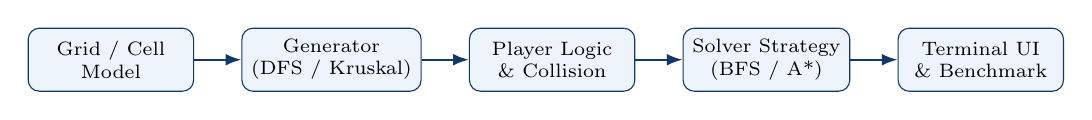
\begin{tikzpicture}[
node distance=6mm,
box/.style={
rectangle,
rounded corners,
draw=GEUBlue,
fill=GEULightBlue,
minimum width=2.10cm,
minimum height=8mm,
align=center,
font=\scriptsize
},
arrow/.style={
-{Latex[length=2mm]},
thick,
draw=GEUBlue
}
]

\node[box] (a) {Grid / Cell\\Model};
\node[box,right=of a] (b) {Generator\\(DFS / Kruskal)};
\node[box,right=of b] (c) {Player Logic\\\& Collision};
\node[box,right=of c] (d) {Solver Strategy\\(BFS / A*)};
\node[box,right=of d] (e) {Terminal UI\\\& Benchmark};

\draw[arrow] (a)--(b);
\draw[arrow] (b)--(c);
\draw[arrow] (c)--(d);
\draw[arrow] (d)--(e);

\end{tikzpicture}

\end{center}

\vspace{3mm}

\begin{columns}[T,totalwidth=\textwidth]

\column{.48\textwidth}

\textbf{\color{GEUBlue}Major Components}

\begin{itemize}\itemsep2pt
\item \texttt{Maze} \& \texttt{Cell}: Grid topology \& walls.
\item \texttt{MazeGenerator}: Abstract generation strategy.
\item \texttt{MazeSolver}: Abstract pathfinding strategy.
\end{itemize}

\column{.48\textwidth}

\textbf{\color{GEUBlue}Changes Since Phase-I}

\begin{itemize}\itemsep2pt
\item Centralized wall mutation interface.
\item Explicit stack iteration for DFS generation.
\item Unified benchmarking metric payload.
\end{itemize}

\end{columns}

\vfill

\smallnote{
Brief Discussion: System architecture uses the Strategy Pattern to decouple generation and pathfinding algorithms.
}

\end{frame}

% ============================================================
% SLIDE 6
% ============================================================
\begin{frame}{Module Design \& Functional Requirements}
\setbeamerfont{itemize/enumerate body}{size=\footnotesize}

\begin{columns}[T,totalwidth=\textwidth]

\column{.42\textwidth}

\textbf{\color{GEUBlue}Major Modules}

\begin{enumerate}\itemsep3pt
\item Grid Engine (\texttt{Cell}, \texttt{Maze})
\item Generators (\texttt{DFSGenerator}, \texttt{Kruskal})
\item Interactive Controls (\texttt{Player})
\item Solvers (\texttt{BFSSolver}, \texttt{AStarSolver})
\end{enumerate}

\column{.54\textwidth}

\textbf{\color{GEUBlue}Functional Requirements}

\begin{itemize}\itemsep3pt
\item Guarantee grid connectivity without closed loops.
\item Validate movement boundaries against cell walls.
\item Construct shortest paths via BFS parent maps.
\item Benchmarking steps, evaluated cells, \& execution time.
\end{itemize}

\end{columns}

\vspace{2mm}

\begin{block}{Module Dependency}
\small Generators and Solvers depend strictly on \texttt{Maze} via abstract strategy interfaces without internal coupling.
\end{block}

\vfill

\smallnote{
Brief Discussion: Explains module separation and interface contracts.
}

\end{frame}

% ============================================================
% SLIDE 7
% ============================================================
\begin{frame}{Technology Stack \& Development Methodology}

\begin{columns}[T,totalwidth=\textwidth]

\column{.48\textwidth}

\begin{block}{Technology Stack}

\begin{itemize}\itemsep2pt
\item \textbf{Language:} C++ (ISO C++17 Standard)
\item \textbf{Data Structures:} \texttt{std::vector}, \texttt{std::priority\_queue}, \texttt{std::stack}, Custom DSU
\item \textbf{Build Tool:} \texttt{g++} / CMake
\item \textbf{Version Control:} Git \& GitHub
\item \textbf{Optional GUI:} SDL2 (Stretch Goal)
\end{itemize}

\end{block}

\column{.48\textwidth}

\begin{block}{Development Methodology}

\begin{enumerate}\itemsep2pt
\item Interface Contracts \& Core Data Models
\item Iterative Generation \& Traversal Solvers
\item Terminal Display \& Interactive Controls
\item Metrics Engine \& Benchmark Tests
\item Validation \& Documentation
\end{enumerate}

\end{block}

\end{columns}

\vfill

\smallnote{
Brief Discussion: Selected C++17 for performance, low memory footprint, and object-oriented abstraction.
}

\end{frame}

% ============================================================
% SLIDE 8
% ============================================================
\begin{frame}{Implementation of PBL Course Concepts}

\scriptsize

\begin{center}

\renewcommand{\arraystretch}{1.25}

\begin{tabularx}{.96\textwidth}
{@{}>{\bfseries\RaggedRight}p{3.2cm}Y R{3.4cm}@{}}

\toprule
Course & Concepts Actually Implemented & Project Module\\
\midrule

Data Structures in C / C++ &
Explicit Stacks, Queue Traversals, Priority Queues, Disjoint Set Union (DSU), 2D Array Grids &
\texttt{DFSGenerator}, \texttt{BFSSolver}, \texttt{AStarSolver}, \texttt{DisjointSet}\\

\midrule

OOPs with C++ &
Abstract Interfaces, Strategy Pattern, Class Encapsulation, Polymorphism, RAII &
\texttt{MazeGenerator}, \texttt{MazeSolver}, \texttt{Maze}, \texttt{Player}\\

\bottomrule

\end{tabularx}

\end{center}

\vfill

\begin{center}
\colorbox{GEULightBlue}{
\parbox{.88\textwidth}{
\centering
\textbf{Important:}
Integrates C++ OOP abstractions directly with foundational C/C++ graph algorithms in a single system.
}}
\end{center}

\smallnote{
Brief Discussion: Technical mapping of course concepts to operational codebase modules.
}

\end{frame}

% ============================================================
% SLIDE 9
% ============================================================
\begin{frame}{Development \& Implementation Progress}

\scriptsize

\begin{center}

\renewcommand{\arraystretch}{1.05}

\begin{tabularx}{.96\textwidth}
{@{}R{3.0cm}R{1.8cm}Y@{}}

\toprule
\textbf{Module} &
\textbf{Status} &
\textbf{Work Completed}\\
\midrule

Grid \& Cell Models &
Completed &
2D grid representation, wall operations, boundary check methods\\

DFS Generator &
Completed &
Iterative stack-based backtracking maze generator\\

BFS Solver &
Completed &
Breadth-first search with parent tracking \& path reconstruction\\

Player Movement &
Completed &
Keypress controls with collision rejection against active walls\\

A* Pathfinder &
In Progress &
Priority queue configuration with Manhattan distance heuristic\\

Kruskal Generator &
In Progress &
Shared wall list setup with Disjoint Set Union (DSU) cycle prevention\\

\bottomrule

\end{tabularx}

\end{center}

\vspace{2mm}

\begin{center}
\colorbox{GEULightBlue}{
\parbox{.65\textwidth}{
\centering
\textbf{Overall Project Completion:}
\textbf{65\% Completed}
}}
\end{center}

\vfill

\smallnote{
Brief Discussion: Core interactive loop and primary graph algorithms are functional.
}

\end{frame}

% ============================================================
% SLIDE 10
% ============================================================
\begin{frame}{Working Prototype / Demonstration}

\begin{columns}[T,totalwidth=\textwidth]

\column{.48\textwidth}

\textbf{\color{GEUBlue}Implemented Features}

\begin{itemize}\itemsep3pt
\item Dynamic maze grid generation (Randomized DFS).
\item Real-time player navigation in terminal.
\item Collision checks rejecting movement into walls.
\item Automated BFS path reconstruction.
\end{itemize}

\column{.48\textwidth}

\begin{block}{Terminal Interface Output}

\ttfamily\scriptsize
+---+---+---+---+---+\\
| P |   |       |   | \quad (P = Player)\\
+   +   +---+   +   +\\
|   |   | G |   |   | \quad (G = Goal)\\
+---+   +   +   +---+\\
|       |           | \quad (* = BFS Path)\\
+---+---+---+---+---+

\vspace{2mm}
\sffamily\scriptsize
\textbf{Status:} Core generate $\rightarrow$ play $\rightarrow$ solve loop fully operational.

\end{block}

\end{columns}

\vfill

\smallnote{
Brief Discussion: Terminal UI displays generated maze, player position, and path solution.
}

\end{frame}

% ============================================================
% SLIDE 11
% ============================================================
\begin{frame}{Testing, Results \& Validation}
\vspace{-3.5mm}

\scriptsize

\begin{center}

\renewcommand{\arraystretch}{1.0}

\begin{tabularx}{\textwidth}
{@{}R{2.4cm}Y Y R{1.2cm}@{}}

\toprule
Test / Module &
Expected Result &
Observed Result &
Status\\
\midrule

Maze Connectivity (DFS) &
All cells accessible from start position &
Zero isolated cells detected across grids &
Pass\\

Wall Collision (Player) &
Invalid moves into walls rejected &
Player position remains unchanged &
Pass\\

BFS Path Validity &
Continuous valid path ending at goal &
Path matches optimal grid traversal &
Pass\\

A* \& Kruskal Tests &
A* path optimality \& Kruskal span &
Implementation phase &
Pending\\

Comparative Benchmarking &
Fair performance comparison &
Scheduled post metrics implementation &
Pending\\

\bottomrule

\end{tabularx}

\end{center}

\vspace{0mm}

\begin{block}{Results / Validation}
\footnotesize Structural validation tests pass; algorithm comparative evaluation planned upon completing A* and Kruskal modules.
\end{block}

\smallnote{
Brief Discussion: Validation suite verifies grid connectivity and player movement logic.
}

\end{frame}

% ============================================================
% SLIDE 12
% ============================================================
\begin{frame}{GitHub Repository \& Development Activity}

\begin{columns}[T,totalwidth=\textwidth]

\column{.46\textwidth}

\textbf{\color{GEUBlue}Repository Information}

\begin{itemize}\itemsep3pt
\item Repository Branch: \texttt{main}
\item README.md: Architecture \& Build Setup Included
\item Contributors: All Team Members Added
\item Active Language: C++ (100\%)
\end{itemize}

\column{.50\textwidth}

\textbf{\color{GEUBlue}Important Commits}

\begin{itemize}\itemsep3pt
\item \texttt{a1b2c3d} Implement Cell \& Maze classes
\item \texttt{e4f5g6h} Add iterative Randomized DFS
\item \texttt{i7j8k9l} Add Player movement \& collision
\item \texttt{m0n1o2p} Add BFS pathfinding solver
\end{itemize}

\end{columns}

\vfill

\begin{center}
\colorbox{GEULightBlue}{
\parbox{.88\textwidth}{
\centering
\textbf{Requirement:}
Individual commits maintained across all members following modular task distribution.
}}
\end{center}

\smallnote{
Brief Discussion: Repository commit history reflects structured modular development.
}

\end{frame}

% ============================================================
% SLIDE 13
% ============================================================
\begin{frame}{Individual Contribution}

\scriptsize

\begin{center}

\renewcommand{\arraystretch}{1.35}

\begin{tabularx}{.96\textwidth}
{@{}R{2.2cm}R{1.8cm}Y R{1.6cm}@{}}

\toprule
Member &
Role &
Technical Contribution &
GitHub Commits\\
\midrule

Tanmay Kumar &
Team Lead &
Grid architecture, abstract strategy interfaces, execution flow loop, statistics engine &
\ph{XX}\\

Sparsh Saxena &
Core Developer &
Iterative DFS generator, BFS solver with parent maps, A* pathfinder implementation &
\ph{XX}\\

Hemang Sethi &
UI / Developer &
Player input mechanics, collision checking, terminal UI rendering, DSU class &
\ph{XX}\\

\bottomrule

\end{tabularx}

\end{center}

\vspace{3mm}

\begin{block}{Individual Evaluation}
Every team member has engineered and verified their assigned codebase modules independently.
\end{block}

\smallnote{
Brief Discussion: Technical contributions map directly to individual commits and modules.
}

\end{frame}

% ============================================================
% SLIDE 14
% ============================================================
\begin{frame}{Challenges, Remaining Work \& Phase-III Roadmap}
\setbeamerfont{itemize/enumerate body}{size=\footnotesize}

\begin{columns}[T,totalwidth=\textwidth]

\column{.48\textwidth}

\textbf{\color{GEUBlue}Challenges Faced}

\begin{itemize}\itemsep2pt
\item Shared wall mutation inconsistencies.
\item Risk of call-stack overflow in DFS.
\item Representing cell-based walls in Kruskal.
\end{itemize}

\vspace{2mm}

\textbf{\color{GEUBlue}Solutions Adopted}

\begin{itemize}\itemsep2pt
\item Funneled wall changes via \texttt{Maze} methods.
\item Switched to explicit heap-allocated stack.
\item Filtered edge creation to right/bottom cells.
\end{itemize}

\column{.48\textwidth}

\textbf{\color{GEUBlue}Phase-III Roadmap}

\begin{enumerate}\itemsep3pt
\item Complete A* solver and Kruskal DSU module.
\item Build metrics engine \& comparison menu.
\item Run comprehensive test suite.
\item Final presentation \& SDL2 GUI (optional).
\end{enumerate}

\end{columns}

\vfill

\smallnote{
Brief Discussion: Addresses current technical roadblocks and outlines clear steps toward final project completion.
}

\end{frame}

% ============================================================
% SLIDE 15
% ============================================================
\begin{frame}{Expected Outcomes \& References}

\begin{columns}[T,totalwidth=\textwidth]

\column{.47\textwidth}

\textbf{\color{GEUBlue}Expected Final Outcomes}

\begin{itemize}\itemsep3pt
\item Fully functional C++ console application.
\item Side-by-side performance benchmarking.
\item Plug-and-play strategy architecture.
\item Interactive human vs algorithm comparison.
\end{itemize}

\column{.47\textwidth}

\textbf{\color{GEUBlue}References}

\begin{enumerate}\itemsep3pt
\item Cormen, T. H., et al. \textit{Introduction to Algorithms}. MIT Press.
\item Gamma, E., et al. \textit{Design Patterns}. Addison-Wesley.
\item ISO/IEC C++17 Standard Specifications.
\end{enumerate}

\vfill

\begin{center}

\colorbox{GEUBlue}{
\parbox{.78\textwidth}{
\centering
\color{white}
\textbf{Thank You}\\
Questions \& Suggestions
}}

\end{center}

\end{columns}

\vfill

\smallnote{
Brief Discussion: Summary of final deliverables and core academic resources used.
}

\end{frame}

\end{document}